\documentclass[11pt,a4paper]{article}
\usepackage[margin=2.5cm]{geometry}
\usepackage{amsmath, amssymb, graphicx, booktabs}
\usepackage[hidelinks]{hyperref}
\setlength{\parindent}{0pt}
\setlength{\parskip}{0.6em}

\title{How much of a shape does a person have?\\[0.3em]\large The shape score, step by step}
\date{4 November 2026}

\begin{document}
\maketitle

\section*{Do I need to understand this?}
You need the \emph{idea}, not the algebra. The idea is three sentences:
\begin{enumerate}
  \item The score is the amount of a shape that, added to the average person, matches the person
        as closely as possible.
  \item It is found by multiplying the person's deviation by the shape at every position and adding
        the products up.
  \item The larger the score (plus or minus), the more of the person's deviation that shape explains.
\end{enumerate}
That is enough to read the figures, the model weights and the results. The algebra in
Section~\ref{sec:why} shows \emph{why} the three sentences hold. It is useful if a supervisor asks,
but in the thesis it is enough to say that the scores are functional principal component scores and
cite the method.

\section{The ingredients}
Take one segment and one person. Along the segment, at positions $s$ from 0 (start) to 1 (end):
\begin{itemize}
  \item $d(s)$, the \textbf{deviation}: the person's turning angle minus the average person's
        turning angle at position $s$. Positive means the person turns more than average there.
  \item $\varphi(s)$, the \textbf{shape}: one fixed curve, found once from everybody. It is scaled so
        that $\sum_s \varphi(s)^2 = 1$; this only fixes its size and has no other meaning.
  \item $c$, the \textbf{score}: one number for this person. It is what we want to find.
\end{itemize}

To keep it small, use only three positions: start, middle and end.

\begin{center}
\begin{tabular}{lrrr}
  \toprule
  position & start & middle & end \\
  \midrule
  deviation $d$ & $3$ & $1$ & $-2$ \\
  shape $\varphi$ & $0.6$ & $0$ & $-0.8$ \\
  \bottomrule
\end{tabular}
\end{center}

The person turns more than average at the start and less at the end. The shape says ``more at the
start, less at the end'' (it crosses zero in the middle). Check the size: $0.6^2 + 0^2 + 0.8^2 = 1$.
(Units of $d$ are left out: think of $3$ as $0.003$\,rad/mm.)

\section{Trying amounts of the shape}
We look for the amount $c$ such that $c \times \varphi$ is as close as possible to $d$.
For a given $c$, the miss at each position is $d - c\,\varphi$. We square the misses (so misses above
and below count the same) and add them:
\[
  \text{error}(c) = \sum_s \bigl(d(s) - c\,\varphi(s)\bigr)^2 .
\]

Try $c = 2$: $c\,\varphi = (1.2,\; 0,\; -1.6)$, misses $= (1.8,\; 1,\; -0.4)$,
error $= 3.24 + 1 + 0.16 = 4.4$.

Doing this for several amounts:

\begin{center}
\begin{tabular}{lrrrrrrr}
  \toprule
  amount $c$ & 0 & 1 & 2 & 3 & \textbf{3.4} & 4 & 5 \\
  error & 14 & 8.2 & 4.4 & 2.6 & \textbf{2.44} & 2.8 & 5 \\
  \bottomrule
\end{tabular}
\end{center}

The error first falls, reaches its lowest value at $c = 3.4$, and rises again: too little of the shape
leaves the deviation unexplained, too much overshoots. This is the U-shaped curve in column 4 of the
week 10 figures. \textbf{The score is the bottom of that U: here $c = 3.4$.}

\section{The shortcut: multiply and add}
Instead of trying many amounts, multiply $d$ and $\varphi$ at each position and add:
\[
  c = \sum_s d(s)\,\varphi(s) = 3 \times 0.6 \;+\; 1 \times 0 \;+\; (-2) \times (-0.8)
    = 1.8 + 0 + 1.6 = 3.4 .
\]
The same number as the bottom of the U. Note what each position did:
\begin{itemize}
  \item start: $d$ and $\varphi$ both positive, the product is positive and \emph{adds};
  \item middle: $\varphi = 0$, the position \emph{does not count};
  \item end: $d$ and $\varphi$ both negative, the product is positive and also \emph{adds}.
\end{itemize}
A position where $d$ and $\varphi$ had opposite signs would have subtracted.

\section{Why the shortcut gives the bottom of the U}
\label{sec:why}
Write out the square:
\[
  \text{error}(c) = \sum_s d^2 \;-\; 2c \sum_s d\,\varphi \;+\; c^2 \sum_s \varphi^2 .
\]
The shape has size 1, $\sum_s \varphi^2 = 1$, so
\[
  \text{error}(c) = \underbrace{\textstyle\sum_s d^2}_{14} \;-\; 2c\,\underbrace{\textstyle\sum_s d\,\varphi}_{3.4} \;+\; c^2 .
\]
This is a parabola in $c$. Its lowest point is where its slope is zero:
\[
  -2 \times 3.4 + 2c = 0 \quad\Longrightarrow\quad c = 3.4 = \sum_s d\,\varphi .
\]

\section{How much of the person the shape explains}
Put the score back in:
\[
  \text{smallest error} = \sum_s d^2 - c^2 = 14 - 3.4^2 = 14 - 11.56 = 2.44 .
\]
The person's total deviation is $\sum_s d^2 = 14$. The shape removes $c^2 = 11.56$ of it, so it explains
\[
  \frac{c^2}{\sum_s d^2} = \frac{11.56}{14} = 83\,\% \text{ of this person's deviation.}
\]
What is left (2.44, or 17\,\%) is column 5 of the figures.

\section{More than one shape}
Add two more shapes, each of size 1 and perpendicular to the others (the products of any two, added
over the positions, are zero):

\begin{center}
\begin{tabular}{lrrrr}
  \toprule
  & start & middle & end & score $c = \sum d\,\varphi$ \\
  \midrule
  deviation $d$ & $3$ & $1$ & $-2$ & \\
  $\varphi_1$ & $0.6$ & $0$ & $-0.8$ & $3.4$ \\
  $\varphi_2$ & $0.8$ & $0$ & $0.6$ & $2.4 - 1.2 = 1.2$ \\
  $\varphi_3$ & $0$ & $1$ & $0$ & $1$ \\
  \bottomrule
\end{tabular}
\end{center}

Each score is found on its own, with the same multiply-and-add. Their squares add up to the whole
deviation:
\[
  3.4^2 + 1.2^2 + 1^2 = 11.56 + 1.44 + 1 = 14 = \sum_s d^2 .
\]
So the three shapes explain 83\,\%, 10\,\% and 7\,\% of this person, and together all of it. With
fewer shapes than positions (as in practice: 3 shapes, 50 positions) some deviation is always left
over.

And the scores rebuild the deviation: $3.4\,\varphi_1 + 1.2\,\varphi_2 + 1\,\varphi_3
= (2.04 + 0.96,\; 1,\; -2.72 + 0.72) = (3,\; 1,\; -2) = d$.

\section{What goes into the risk model}
Only the scores. With three shapes each person enters the model as three numbers, and the model learns
one weight per shape:
\[
  \mathrm{cloglog}(p) = a + g\,\mathrm{SCORE2} + b_1 c_1 + b_2 c_2 + b_3 c_3 .
\]
$b_k > 0$ means that people with more of shape $k$ developed plaque more often.

\section{On the real figures}
The week 10 figure below does exactly this with 400 positions instead of three. Column 3 shows $d$ and
$c\,\varphi$, column 4 the error for each amount (the U), and column 5 what is left after removing
each shape.

\begin{center}
  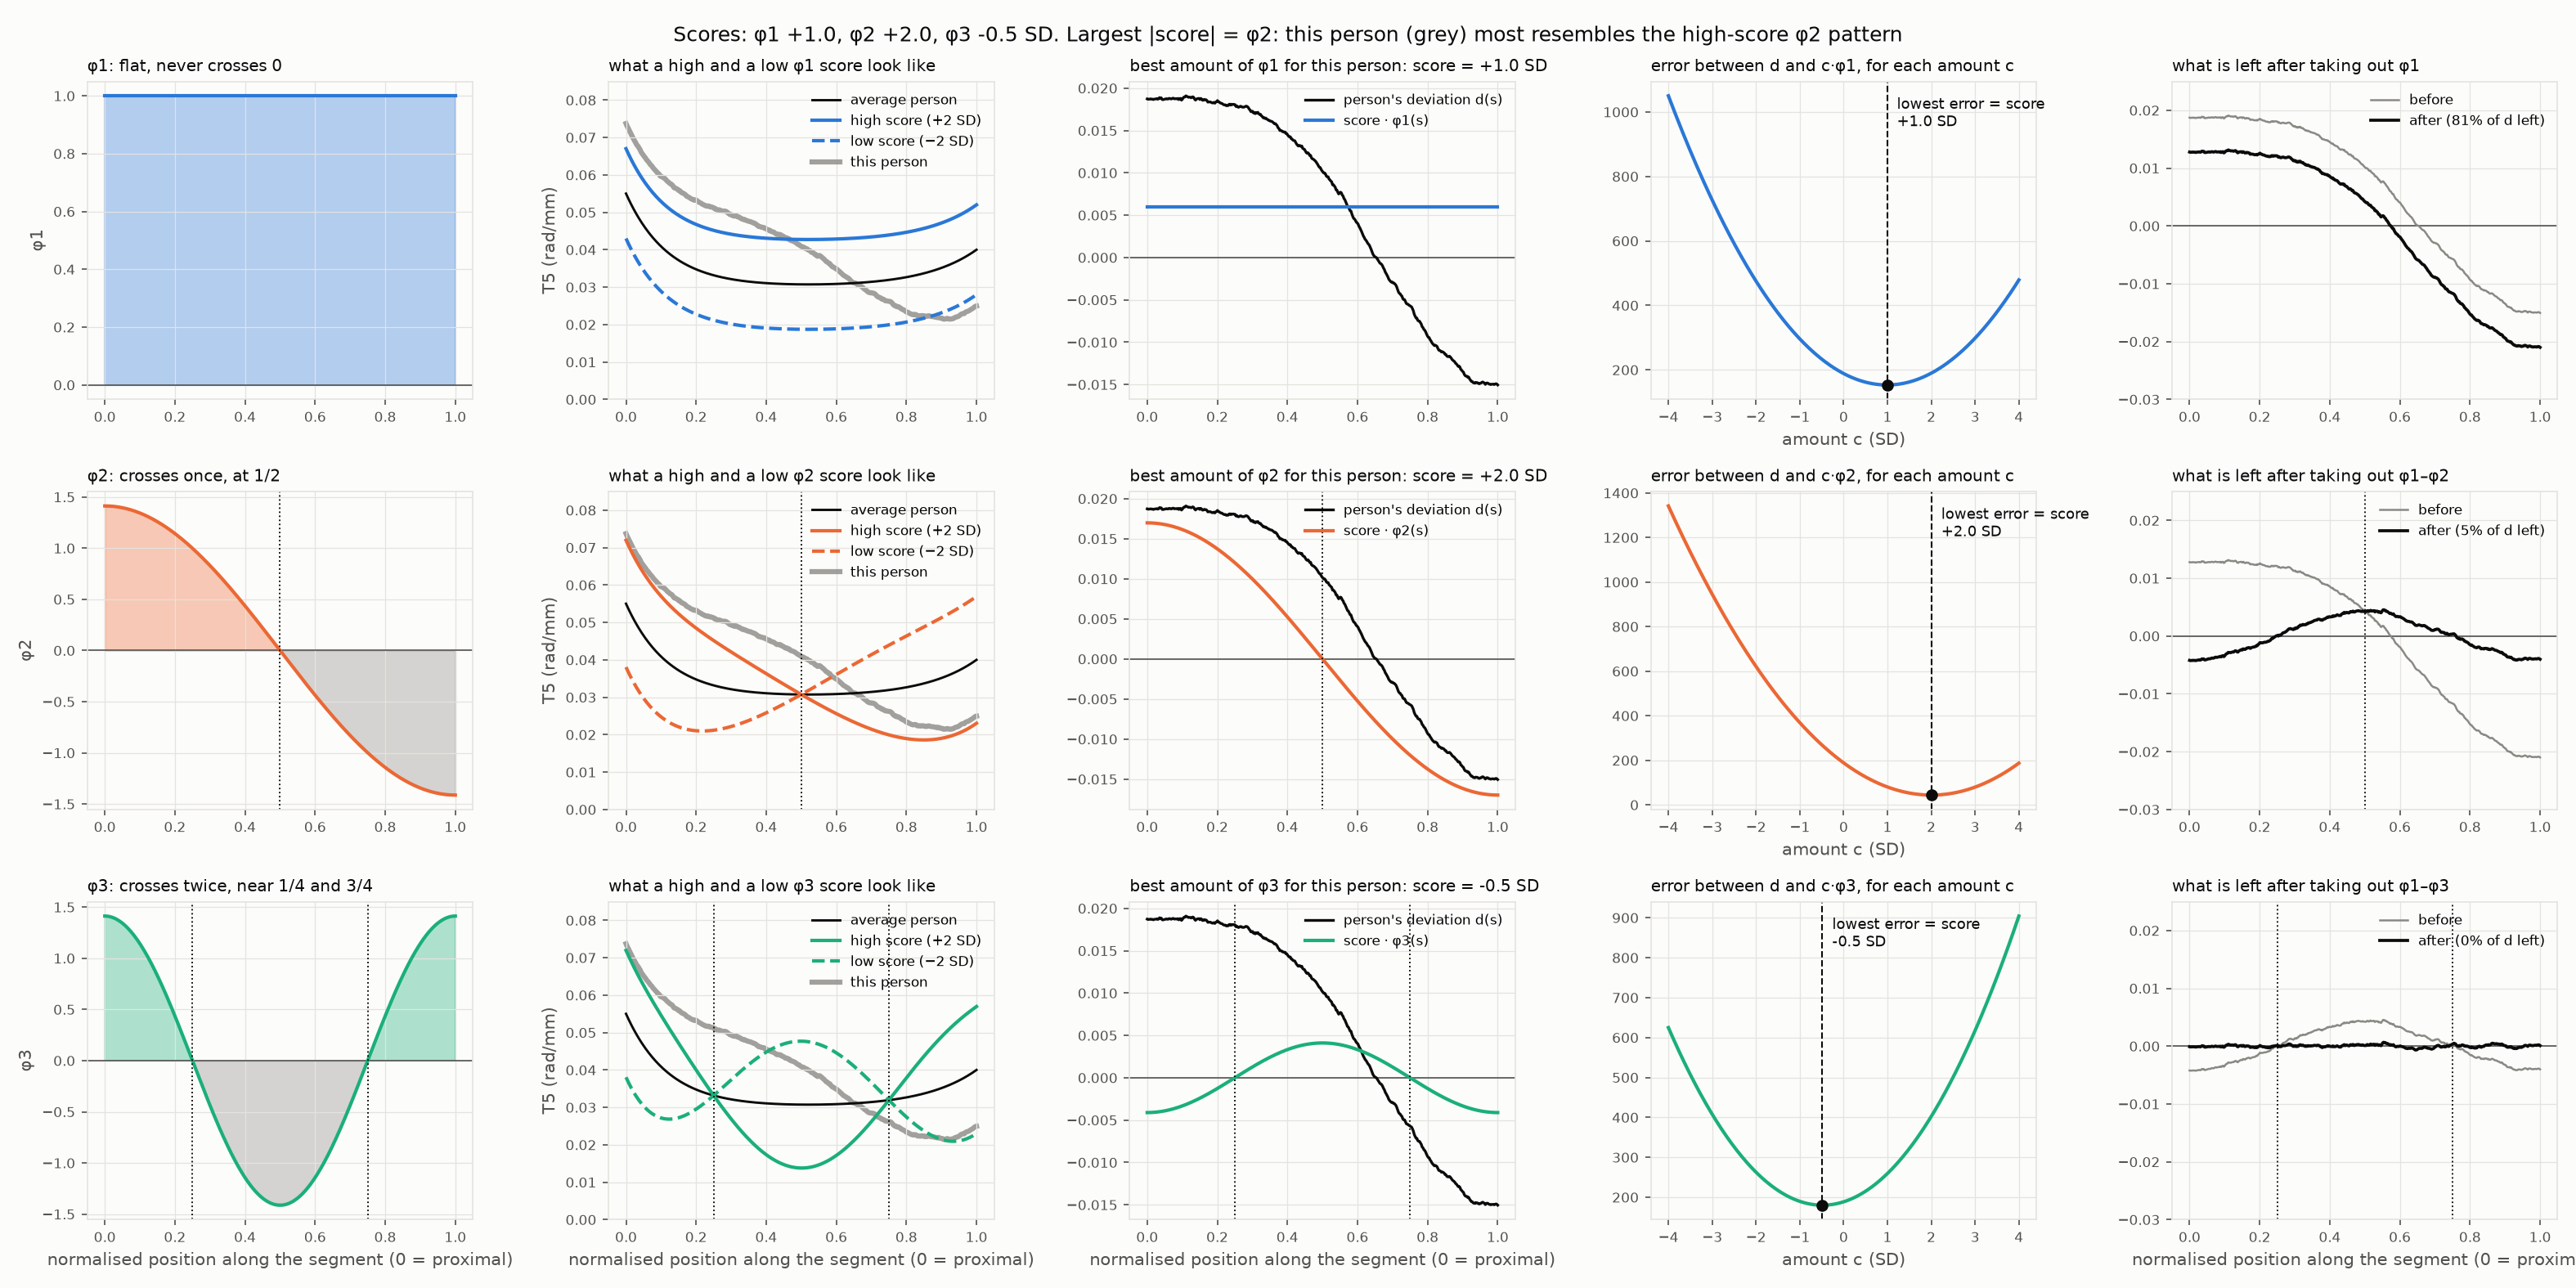
\includegraphics[width=\textwidth]{week_figure/shape_scores_phi2_person.png}
\end{center}

\end{document}
